\documentclass[conference,letterpaper]{IEEEtran}
\IEEEoverridecommandlockouts
% Toque MCIC sobre IEEEtran: solo color y diagramas. No cambia márgenes,
% fuentes, columnas ni tamaños de la plantilla IEEE.
% tectonic compila con XeTeX: Times New Roman (la de IEEE y la secundaria del manual UD)
% se lee de las fuentes del manual de marca; si no está, TeX Gyre Termes (clon de Times).
\usepackage{amsmath,amssymb}
\usepackage{newtxmath}
\usepackage{fontspec}
\providecommand{\UDmarca}{/Users/juferoga/repos/ud/maestria/mcic/.UniversidadDistrital-manual-marca}
\IfFileExists{\UDmarca/fuentes/times.ttf}{%
  \setmainfont{times.ttf}[Path=\UDmarca/fuentes/, BoldFont=timesbd.ttf,
    ItalicFont=timesi.ttf, BoldItalicFont=timesbi.ttf]}{%
  \setmainfont{texgyretermes}[Extension=.otf, UprightFont=*-regular, BoldFont=*-bold,
    ItalicFont=*-italic, BoldItalicFont=*-bolditalic]}
\setmonofont{texgyrecursor}[Extension=.otf, UprightFont=*-regular, BoldFont=*-bold, Scale=0.95]
\usepackage[spanish,es-noshorthands,es-tabla,es-nolists]{babel}
\usepackage{graphicx}
\usepackage{booktabs,tabularx,array,multirow}
\usepackage[table]{xcolor}
\usepackage{tikz}
\usetikzlibrary{positioning,arrows.meta,calc,fit}
\usepackage[hidelinks]{hyperref}
\usepackage{cite}
\usepackage{url}

% Paleta del manual de marca UD (design.md)
\definecolor{udazul}{HTML}{1291C0}
\definecolor{udazulosc}{HTML}{0C6F96}
\definecolor{uddorado}{HTML}{B49739}
\definecolor{udverde}{HTML}{00A859}
\definecolor{udplata}{HTML}{98999A}
\definecolor{udsable}{HTML}{373435}
\definecolor{udrojo}{HTML}{ED3237}

\hypersetup{colorlinks=true,linkcolor=udazulosc,citecolor=udazulosc,urlcolor=udazulosc}

% Bloques de la ecuación de búsqueda: el mismo color en ecuación, PRISMA y matriz.
\newcommand{\bloqueA}[1]{\textcolor{udazulosc}{#1}}
\newcommand{\bloqueB}[1]{\textcolor{uddorado!85!black}{#1}}
\newcommand{\bloqueC}[1]{\textcolor{udverde!80!black}{#1}}
\newcommand{\etiqueta}[2]{\tikz[baseline=(t.base)]\node[fill=#1,text=white,inner sep=1.6pt,
  rounded corners=1pt,font=\bfseries\scriptsize](t){#2};}

% Cabecera de tablas: filete azul y fila sombreada clara
\newcommand{\cabecera}{\rowcolor{udazul!12}}
\arrayrulecolor{udazulosc}

% Columnas de la matriz
\newcolumntype{L}[1]{>{\raggedright\arraybackslash}p{#1}}
\newcolumntype{Y}{>{\raggedright\arraybackslash}X}

\makeatletter
\providecommand{\filas}[1]{\@@input #1 }
\makeatother

% Marca de enfoque en la matriz (A..E)
\newcommand{\enf}[1]{\textcolor{udazulosc}{\bfseries #1}}

% Cajas del PRISMA
\tikzset{
  caja/.style={draw=udazulosc,line width=0.5pt,rounded corners=1.5pt,align=center,
    font=\scriptsize,inner sep=2.5pt,text width=#1},
  caja/.default=3.6cm,
  excl/.style={draw=udplata,line width=0.5pt,rounded corners=1.5pt,align=left,
    font=\scriptsize,inner sep=2.5pt,fill=udplata!8,text width=#1},
  excl/.default=2.75cm,
  fase/.style={fill=udazul,text=white,font=\bfseries\tiny,minimum width=0.42cm,
    rounded corners=1pt,inner sep=1pt},
  flecha/.style={-{Latex[length=1.6mm]},udsable,line width=0.5pt},
}

% Generado por revision/generar_e1.py; no editar a mano.
\newcommand{\nArxivQuno}{35}
\newcommand{\nArxivQdos}{3}
\newcommand{\nArxivTotal}{38}
\newcommand{\nArxivDup}{0}
\newcommand{\nOaQuno}{162}
\newcommand{\nOaQdos}{33}
\newcommand{\nOaTotal}{195}
\newcommand{\nOaDup}{39}
\newcommand{\nDup}{39}
\newcommand{\nTamizados}{194}
\newcommand{\nExclTitulo}{147}
\newcommand{\nPasan}{47}
\newcommand{\nExclTexto}{10}
\newcommand{\nIncluidosBases}{37}
\newcommand{\nOtros}{21}
\newcommand{\nTotalIncluidos}{58}
\newcommand{\nMatriz}{16}
\newcommand{\nMatrizRecientes}{13}
\newcommand{\nRecientes}{49}
\newcommand{\nTextoCompleto}{35}
\newcommand{\nSoloResumen}{23}
\newcommand{\fechaConsulta}{2026-11-06}
\newcommand{\fechaConsultaOa}{2026-11-07}

% Generado por articulo/generar_cifras.py; no editar a mano.
\newcommand{\cifCommits}{612.811}
\newcommand{\cifDesarrollo}{558.438}
\newcommand{\cifPrueba}{54.373}
\newcommand{\cifPrevMin}{3{,}9\,\%}
\newcommand{\cifPrevMax}{4{,}5\,\%}
\newcommand{\cifPrevAnioVeintiseis}{3{,}39\,\%}
\newcommand{\cifPositivosDesarrollo}{23.735}
\newcommand{\cifPositivosPrueba}{1.947}
\newcommand{\cifCensurados}{26.133}
\newcommand{\cifAutores}{18.127}
\newcommand{\cifSubsistemas}{748}
\newcommand{\cifNVariables}{22}
\newcommand{\cifPrevQunoAdd}{0{,}9\,\%}
\newcommand{\cifPrevQcincoAdd}{11{,}7\,\%}
\newcommand{\cifReviewedIni}{0{,}42}
\newcommand{\cifReviewedFin}{0{,}71}
\newcommand{\cifFixIni}{14{,}5\,\%}
\newcommand{\cifFixFin}{18{,}4\,\%}
\newcommand{\cifValMayoritaria}{0{,}0410}
\newcommand{\cifValLogistica}{0{,}1486}
\newcommand{\cifValGB}{0{,}1578}
\newcommand{\cifParamGB}{5.645}
\newcommand{\cifParamLR}{23}
\newcommand{\cifNConfigsRef}{10}
\newcommand{\cifValFE}{0{,}1495}
\newcommand{\cifValFEde}{0{,}0053}
\newcommand{\cifValVariante}{0{,}1206}
\newcommand{\cifReglasMin}{3}
\newcommand{\cifReglasMax}{6}
\newcommand{\cifAntMin}{3}
\newcommand{\cifAntMax}{10}
\newcommand{\cifTiempoFE}{11}
\newcommand{\cifNBusqueda}{14}
\newcommand{\cifMejorBusqueda}{0{,}1485}
\newcommand{\cifRazonValFE}{94{,}8\,\%}
\newcommand{\cifCongelada}{2026-11-07 23:41}
\newcommand{\cifHuella}{11e7039f3cc27912}
\newcommand{\cifSemillaRef}{11}
\newcommand{\cifSensMax}{0{,}1498}
\newcommand{\cifSensMaxR}{10}
\newcommand{\cifSensMaxPm}{0{,}05}
\newcommand{\cifSensMin}{0{,}1305}
\newcommand{\cifSensMinR}{15}
\newcommand{\cifSensMinPm}{0{,}30}
\newcommand{\cifSensMutBaja}{0{,}1486}
\newcommand{\cifSensMutAlta}{0{,}1347}
\newcommand{\cifReglasVariante}{15}
\newcommand{\cifAntVariante}{29}
\newcommand{\cifRegReferencias}{30}
\newcommand{\cifRegPropuesto}{84}
\newcommand{\cifRegBusq}{42}
\newcommand{\cifRegSens}{24}
\newcommand{\cifTestMay}{0{,}0346}
\newcommand{\cifTestMayde}{0{,}0000}
\newcommand{\cifTestMayic}{[0{,}033;\ 0{,}036]}
\newcommand{\cifCaidaMay}{15{,}5\,\%}
\newcommand{\cifTestLR}{0{,}1274}
\newcommand{\cifTestLRde}{0{,}0000}
\newcommand{\cifTestLRic}{[0{,}117;\ 0{,}140]}
\newcommand{\cifCaidaLR}{14{,}2\,\%}
\newcommand{\cifTestGB}{0{,}1320}
\newcommand{\cifTestGBde}{0{,}0007}
\newcommand{\cifTestGBic}{[0{,}121;\ 0{,}146]}
\newcommand{\cifCaidaGB}{16{,}3\,\%}
\newcommand{\cifTestVar}{0{,}0901}
\newcommand{\cifTestVarde}{0{,}0000}
\newcommand{\cifTestVaric}{[0{,}083;\ 0{,}098]}
\newcommand{\cifCaidaVar}{25{,}3\,\%}
\newcommand{\cifTestFE}{0{,}1202}
\newcommand{\cifTestFEde}{0{,}0024}
\newcommand{\cifTestFEic}{[0{,}108;\ 0{,}128]}
\newcommand{\cifCaidaFE}{19{,}5\,\%}
\newcommand{\cifPrevPrueba}{3{,}46\,\%}
\newcommand{\cifNPrueba}{54.373}
\newcommand{\cifCuno}{91{,}1\,\%}
\newcommand{\cifFriedmanP}{0{,}0043}
\newcommand{\cifNemenyiCD}{3{,}05}
\newcommand{\cifAssistedN}{2.031}
\newcommand{\cifAssistedPrev}{2{,}81\,\%}
\newcommand{\cifAssistedLR}{0{,}079}
\newcommand{\cifSinAssistedLR}{0{,}130}
\newcommand{\cifAssistedGB}{0{,}067}
\newcommand{\cifSinAssistedGB}{0{,}136}
\newcommand{\cifAssistedFE}{0{,}055}
\newcommand{\cifSinAssistedFE}{0{,}120}
\newcommand{\cifFEMarcMin}{0{,}0\,\%}
\newcommand{\cifFEMarcMax}{17{,}9\,\%}
\newcommand{\cifFEMccMin}{0{,}000}
\newcommand{\cifFEMccMax}{0{,}175}
\newcommand{\cifFEApMin}{0{,}1172}
\newcommand{\cifFEApMax}{0{,}1245}
\newcommand{\cifFERefMarc}{17{,}9\,\%}
\newcommand{\cifFERefAp}{0{,}1172}
\newcommand{\cifMcAciertaGB}{584}
\newcommand{\cifMcFallaGB}{4.379}
\newcommand{\cifMcAciertaLR}{667}
\newcommand{\cifMcFallaLR}{3.422}
\newcommand{\cifMcAciertaVar}{3.306}
\newcommand{\cifMcFallaVar}{878}
\newcommand{\cifNReglasRef}{5}
\newcommand{\cifParamFE}{27}
\newcommand{\cifParamGBprueba}{5.765}
\newcommand{\cifErrQcincoSens}{86{,}8\,\%}
\newcommand{\cifErrQcincoPrev}{9{,}6\,\%}
\newcommand{\cifErrQunoPrev}{0{,}8\,\%}
\newcommand{\cifErrFixAp}{0{,}088}
\newcommand{\cifErrNoFixAp}{0{,}126}
\newcommand{\cifErrFixSens}{20{,}3\,\%}
\newcommand{\cifErrNoFixSens}{58{,}7\,\%}
\newcommand{\cifMesIni}{0{,}151}
\newcommand{\cifMesFin}{0{,}086}
\newcommand{\cifMesGBIni}{0{,}158}
\newcommand{\cifMesGBFin}{0{,}104}
\newcommand{\cifRangoFE}{2{,}50}
\newcommand{\cifRangoGB}{1{,}00}
\newcommand{\cifRangoLR}{2{,}50}
\newcommand{\cifRangoVar}{4{,}00}
\newcommand{\cifRangoMay}{5{,}00}
\newcommand{\cifAporteEvolPrueba}{33\,\%}
\newcommand{\cifItDosCreOriFE}{0{,}1485}
\newcommand{\cifItDosCreOriGB}{0{,}1578}
\newcommand{\cifItDosCreOriRazon}{0{,}941}
\newcommand{\cifItDosCreAmpFE}{0{,}1472}
\newcommand{\cifItDosCreAmpGB}{0{,}1578}
\newcommand{\cifItDosCreAmpRazon}{0{,}933}
\newcommand{\cifItDosDesOriFE}{0{,}1478}
\newcommand{\cifItDosDesOriGB}{0{,}1577}
\newcommand{\cifItDosDesOriRazon}{0{,}937}
\newcommand{\cifItDosDesAmpFE}{0{,}1428}
\newcommand{\cifItDosDesAmpGB}{0{,}1577}
\newcommand{\cifItDosDesAmpRazon}{0{,}905}
\newcommand{\cifItDosUmbral}{0{,}947}
\newcommand{\cifItDosAdoptada}{no}

\renewcommand{\IEEEkeywordsname}{Palabras clave}
\newcommand{\pendiente}[1]{\textcolor{udrojo}{\textbf{[#1]}}}
\raggedbottom

\begin{document}

\title{¿Sobrevive un clasificador difuso-evolutivo interpretable a la deriva de 2026? Riesgo de los commits del kernel de Linux}

\author{\IEEEauthorblockN{Juan Felipe Rodríguez Galindo}
\IEEEauthorblockA{Maestría en Ciencias de la Información y las Comunicaciones\\
Universidad Distrital Francisco José de Caldas, Bogotá, Colombia\\
Código 20261595004 \textperiodcentered{} Inteligencia Computacional \textperiodcentered{} Artículo final}}

\maketitle

\begin{abstract}
Predecir si un commit tendrá que corregirse permite enfocar la revisión de código. En el kernel de Linux la etiqueta es explícita: el trailer \texttt{Fixes:} de un commit posterior señala al culpable. Se construyó un dataset de \cifCommits{} commits de 2019--2026, minado del historial completo, y se comparó un clasificador de reglas difusas cuyas funciones de pertenencia y reglas ajusta un algoritmo genético con la clase mayoritaria, la regresión logística, el \emph{gradient boosting} y una variante sin evolución. Se usó validación temporal con hueco de 90 días, AUC-PR como métrica principal y una única evaluación en 2026, el año de la etiqueta \texttt{Assisted-by} para contribuciones asistidas por IA. El modelo propuesto no alcanzó el criterio de éxito fijado de antemano: obtuvo \cifTestFE{} de AUC-PR, el \cifCuno{} del \emph{gradient boosting} (meta: 90\,\%), y su caída desde validación (\cifCaidaFE{}) fue mayor que la de la referencia (\cifCaidaGB{}). Aun así, triplica la prevalencia con 3--6 reglas legibles frente a miles de parámetros, y la evolución aporta un \cifAporteEvolPrueba{} sobre la variante sin evolución. Una segunda iteración, decidida solo en validación, no mejoró el modelo.
\end{abstract}

\begingroup\renewcommand{\abstractname}{Abstract}
\begin{abstract}
We build a dataset of \cifCommits{} Linux kernel commits (2019--2026) labelled by later \texttt{Fixes:} trailers and compare a genetically tuned fuzzy rule classifier with majority, logistic regression, gradient boosting and a non-evolved variant, under temporal validation and a single 2026 test. The fuzzy model missed the pre-registered goal: its AUC-PR reached \cifCuno{} of gradient boosting (target 90\,\%) and degraded more under drift, while using only 3--6 readable rules; evolution improved AUC-PR by \cifAporteEvolPrueba{} over the non-evolved variant.
\end{abstract}\endgroup

\begin{IEEEkeywords}
predicción de defectos justo a tiempo, kernel de Linux, deriva temporal, sistemas difusos, computación evolutiva, AUC-PR.
\end{IEEEkeywords}

%=====================================================================
\section{Introducción}

El riesgo de un cambio de software se estima desde hace dos décadas con métricas del propio cambio: cuánto toca, cuánto se difunde y cuánta experiencia tiene su autor \cite{Mockus2000,Kamei2013}. Es la predicción de defectos justo a tiempo (JIT): el aviso llega cuando el cambio aún está en revisión. El kernel de Linux recibe miles de commits por versión y tiene una etiqueta que pocos proyectos tienen: cuando un commit corrige otro, el trailer \texttt{Fixes:} nombra al culpable, sin tener que adivinarlo con \texttt{git blame} como hace SZZ \cite{Sliwerski2005}. En estudios empíricos sobre el trailer \texttt{Fixes:}, el 81\,\% se confirmó como causa del bug; el resto es ambiguo o incorrecto \cite{Lyu2024}.

En 2026 cambió quién escribe parte de esos commits. La versión 7.0 pidió declarar con \texttt{Assisted-by:} la ayuda de asistentes de IA \cite{KernelAdd}. La 7.3 redujo la etiqueta a \texttt{Assisted-by: LLM} \cite{KernelSimpl}. El 14 de octubre se eliminó, porque solo cerca del 10\,\% de los 18\,533 commits de la 7.3 la llevaba, aunque el uso real de LLM es mucho mayor \cite{KernelRemove}. Esto tiene una consecuencia de diseño: la ``era IA'' no se puede definir con la etiqueta, porque que falte no quiere decir que no hubo IA. Se define por fecha, y la etiqueta queda solo para describir un subgrupo, como cota inferior.


\subsection{Problema y pregunta de investigación}

\textbf{Problema.} Clasificar cada commit del kernel como \emph{riesgoso} si un commit posterior lo cita con \texttt{Fixes:} en 90 días o menos, usando solo información disponible en el momento de integrarlo, y con un modelo que un mantenedor pueda leer.

\textbf{Pregunta.} ¿Un clasificador de a lo sumo 15 reglas difusas, cuyas funciones de pertenencia y reglas se ajustan con un algoritmo evolutivo, alcanza en los commits de 2026 un AUC-PR de al menos el 90\,\% del mejor modelo de referencia (regresión logística o \emph{gradient boosting}), y pierde menos AUC-PR que ese modelo al pasar de la validación (ventanas anuales 2023, 2024 y 2025, entrenando desde 2019) a la prueba (enero--julio de 2026)?

\subsection{Criterio de éxito (etapa 1 de CRISP-ML(Q) \cite{Studer2021})}

Sea $\mathrm{AP}_m^{V}$ el AUC-PR medio del modelo $m$ en las ventanas de validación y $\mathrm{AP}_m^{T}$ su AUC-PR en la prueba de 2026, ambos con intervalo de confianza del 95\,\% por \emph{bootstrap}. Sean $\Delta_m=(\mathrm{AP}_m^{V}-\mathrm{AP}_m^{T})/\mathrm{AP}_m^{V}$ la caída relativa, $\pi^{T}$ la prevalencia de positivos en la prueba (el AUC-PR de la clase mayoritaria), FE el modelo propuesto y $R$ la mejor referencia clásica en validación. El proyecto se declara exitoso si se cumplen las tres condiciones de la Tabla~\ref{tab:criterio}. Si no se cumplen, se reporta así, sin volver a ajustar nada con la prueba.

\begin{table}[!t]
\caption{Criterio de éxito, fijado antes de ver los datos}
\label{tab:criterio}
\centering\footnotesize
\begin{tabularx}{\columnwidth}{@{}l Y@{}}
\toprule
\cabecera & \textbf{Condición}\\
\midrule
C1 Desempeño & $\mathrm{AP}_{FE}^{T}\ge 0{,}90\,\mathrm{AP}_{R}^{T}$\\
C2 Robustez & $\Delta_{FE}<\Delta_{R}$ (diferencia observada, con IC 95\,\%)\\
C3 Piso & El IC 95\,\% de $\mathrm{AP}_{FE}^{T}$ excluye $\pi^{T}$; McNemar contra cada referencia con $\alpha=0{,}05$\\
Restricción & $\le$15 reglas y $\le$3 antecedentes por regla\\
\bottomrule
\end{tabularx}
\end{table}

\subsection{Datos y aprobación}
Los datos son públicos: el historial completo de \texttt{torvalds/linux} (GPL-2.0), minado directamente para tener una sola fuente de 2014 a 2026. El dataset de Zenodo de Maes Bermejo \emph{et al.} (más de 90\,000 pares commit corregido--commit que corrige, CC-BY-4.0) \cite{MaesBermejo2024} sirve para contrastar la etiqueta. Por eso no se requiere solicitud de aprobación. Los nombres y correos de los autores se reemplazan por identificadores.%=====================================================================
\section{Estado del arte}

\subsection{Método de búsqueda}
La búsqueda sigue a PRISMA 2020 \cite{Page2021} en versión breve. El problema se descompone en tres bloques, unidos con OR por dentro y AND entre ellos:

\noindent\fbox{\parbox{\dimexpr\columnwidth-2\fboxsep-2\fboxrule}{\footnotesize\raggedright
\etiqueta{udazulosc}{A} \bloqueA{(commit* OR ``code change*'' OR ``software change*'' OR patch* OR ``pull request*'' OR ``Linux kernel'')} AND\\
\etiqueta{uddorado}{B} \bloqueB{(``defect prediction'' OR ``bug prediction'' OR ``bug-introducing'' OR ``bug-inducing'' OR ``fix-inducing'' OR ``just-in-time'' OR ``change risk'' OR ``risk prediction'' OR ``defect-prone'' OR buggy)} AND\\
\etiqueta{udverde}{C} \bloqueC{(fuzzy OR ``rule-based'' OR evolutionary OR ``genetic algorithm'' OR ``genetic programming'' OR ``search-based'' OR interpretab* OR explainab*)}}}

\smallskip
La ecuación Q1 usa los tres bloques. La Q2 cambia el bloque C por uno de deriva temporal (``concept drift'', drift, ``temporal validation'', ``time-aware'', ``realistic evaluation'', ``data shift'', ``distribution shift'', ``time travel''). Ambas se corrieron, limitadas a 2019--2026 y con los comodines expandidos a mano, en arXiv (\fechaConsulta) y en OpenAlex (\fechaConsultaOa, título y resumen), las dos por API pública para que la búsqueda se pueda repetir. OpenAlex, que indexa IEEE, ACM, Springer y Elsevier, reemplaza a Scopus o IEEE Xplore por falta de acceso institucional. Los clásicos anteriores a 2019 y los trabajos encontrados por citas entran como ``otras fuentes''.

Los criterios se escribieron antes del tamizaje. Se incluye un trabajo si (I1) predice el riesgo de un cambio individual o estudia la validez de esa evaluación (orden temporal, latencia, ruido de la etiqueta), (I2) reporta métricas cuantitativas y (I3) describe sus datos. Se excluye si (E1) trata reparación o generación de código, (E2) trabaja solo a nivel de archivo o módulo (se admitieron clasificadores difusos y evolutivos de módulo, porque de commit no hay), (E3) es de otro dominio, (E4) es solo un dataset o (E5) no se puede verificar. Cada trabajo incluido se contrastó con su DOI, la editorial o arXiv: \nTextoCompleto{} se leyeron completos y \nSoloResumen{} solo por resumen o fuentes secundarias. De \nOaTotal{} registros de OpenAlex y \nArxivTotal{} de arXiv, \nPasan{} pasaron el tamizaje por título y resumen y \nIncluidosBases{} se incluyeron tras el texto completo, más \nOtros{} de otras fuentes. El flujo PRISMA y la matriz completa (\nTotalIncluidos{} filas, con la URL consultada) se adjuntan como anexo.



\subsection{Síntesis por enfoques}

\textbf{A. Métricas de cambio y aprendizaje clásico.} El enfoque fundacional usa métricas del cambio con regresión logística \cite{Mockus2000,Kamei2013}. Sigue siendo difícil de superar: con partición cronológica, una regresión logística de una sola variable (líneas añadidas) iguala o supera en AUC a DeepJIT y CC2Vec \cite{Zeng2021}.

\textbf{B. Aprendizaje profundo y LLM.} Las redes sobre el diff y el mensaje y los modelos preentrenados con métricas expertas \cite{Ni2022} marcan la cota alta de AUC-ROC, cerca de 0,88 en JIT-Defects4J. Tienen tres costos para este proyecto: son opacos, se evalúan sobre todo en Java y casi nunca reportan AUC-PR. En la industria, un LLM ya puntúa el riesgo de cada diff, pero su explicación (pesos de atención) convenció a pocos desarrolladores \cite{Liu2026}.

\textbf{C. Interpretabilidad, reglas, difuso y evolutivo.} Los profesionales piden saber por qué se marca un cambio \cite{Jiarpakdee2021}. La respuesta dominante es explicar después una caja negra: LIME en JITLine \cite{JITLine2021}, reglas locales en PyExplainer \cite{PyExplainer2021}, commits similares en IRJIT \cite{Sahar2024}. Esas explicaciones post hoc no son formalmente correctas ni estables, lo que llevó a explicadores con garantías formales \cite{Yu2024FoX}. A nivel de commit, lo evolutivo y lo difuso aparecen solo como piezas auxiliares: evolución diferencial para SMOTE \cite{JITLine2021}, NSGA-II para los coeficientes de una regresión logística \cite{Chen2018MULTI}, búsqueda armónica para hiperparámetros \cite{Kang2021}, un algoritmo genético que pondera variables \cite{Mostafa2025} y Fuzzy C-Means que pondera la atención de una red multitarea \cite{Chen2025}. Los sistemas difusos y neuro-difusos con metaheurísticas existen, pero a nivel de módulo, sobre datos NASA, con particiones aleatorias y exactitud como métrica \cite{Aftab2023,Dey2025}. En \cite{Aftab2023}, por ejemplo, una exactitud del 91\,\% esconde una sensibilidad de 0,33. No se encontró un clasificador de reglas difusas para riesgo de commits.

\textbf{D. Evaluación realista, deriva y latencia.} Los modelos JIT se degradan con el tiempo. En Qt y OpenStack el AUC cae entre 11 y 34 puntos en un año, y reentrenar recupera parte \cite{McIntosh2018}. La validación cruzada es optimista: JITBoost baja de 0,891 a 0,863 de AUC al pasar a partición temporal \cite{Shehab2023}. Desde 2023 la deriva en JIT es una línea activa: detectarla a partir de la interpretación del modelo \cite{Chitsazian2026}, reciclar modelos antiguos \cite{Patel2024}, actualizar de forma continua, que en Ubisoft supera al reentrenamiento periódico \cite{Olewicki2024}, o aprender en línea con espera de la etiqueta \cite{Tian2026}. Ninguno de estos trabajos reporta AUC-PR. La etiqueta llega tarde: el retraso mediano hasta descubrir un defecto va de 15 a 416 días según el proyecto \cite{Cabral2019}, y la espera elegida cambia la medida de desempeño hasta en 25\,\% \cite{Song2023}. La evidencia más cercana a este proyecto viene del propio kernel: al pasar de un conjunto balanceado artificialmente a la prevalencia real, el PR-AUC de ocho técnicas JIT de vulnerabilidades cae de 0,805 a 0,016 \cite{Nguyen2025}. Sobre la era de la IA, los PR de agentes no inducen más bugs que los humanos en un grado relevante, aunque sí cambian el tamaño y el tipo de los cambios \cite{Mazloomzadeh2026}. Es decir, la deriva esperada está en las covariables más que en la tasa de defectos.

\textbf{E. La etiqueta.} SZZ es ruidoso: cerca de la mitad de las correcciones que identifica no lo son \cite{Herbold2022}; filtrarlas con un LLM reduce 21\,\% los commits inductores en PostgreSQL y hace la tarea más difícil de lo reportado \cite{Veras2025}. Sus variantes alcanzan F1 de 0,49--0,51 contra la verdad de \texttt{Fixes:} en Linux \cite{Lyu2024}. Los defectos latentes que aún no se han descubierto bajan la sensibilidad cerca de 90\,\% si no se recorta la cola reciente \cite{Falessi2022}.
\subsection{Brecha}
Los enfoques anteriores dejan cuatro vacíos que este proyecto atiende a la vez:
\begin{enumerate}
\item No hay un clasificador de reglas difusas ajustado con evolución para riesgo a nivel de commit. A ese nivel, lo difuso y lo evolutivo son auxiliares; como clasificador, se quedaron en módulos con particiones aleatorias.
\item La deriva en JIT está demostrada y se estudia activamente \cite{McIntosh2018,Chitsazian2026,Patel2024}, pero no se ha medido con AUC-PR y prevalencia real en commits del kernel etiquetados con \texttt{Fixes:}.
\item Nadie ha medido si la interpretabilidad intrínseca (pocas reglas legibles) cuesta desempeño o, al contrario, da robustez frente a la deriva.
\item 2026 es el primer año en que el kernel pidió declarar la ayuda de IA \cite{KernelAdd}, aunque la etiqueta se retiró en octubre por su bajo uso \cite{KernelRemove}.
\end{enumerate}

%=====================================================================
\section{Metodología: datos y modelos}

La metodología sigue las etapas de CRISP-ML(Q) \cite{Studer2021}. Esta sección cubre la comprensión y preparación de los datos (etapa 2) y la elección de los modelos (etapa 3). Las subsecciones finales declaran el protocolo de evaluación (etapa 3), fijado antes de entrenar el modelo propuesto.

\subsection{Construcción del dataset}

Se minó un clon completo de \texttt{torvalds/linux} con una sola pasada de \texttt{git log} sobre la rama principal, sin commits de fusión, desde 2014. Los años 2014--2018 solo sirven para calcular la experiencia de los autores. Por cada commit se extraen el \emph{numstat} del diff, los trailers del mensaje y las fechas. Las referencias \texttt{Fixes:} (prefijos de al menos 8 caracteres hexadecimales) se resuelven contra el historial: el 9,4\,\% que no se resuelve apunta a commits anteriores a 2014 o a otros árboles.

\textbf{Etiqueta.} Un commit es \emph{riesgoso} si algún commit posterior de la rama principal lo cita con \texttt{Fixes:} en 90 días o menos. Los commits con menos de 90 días de observación a la fecha de corte quedan \emph{censurados} y se excluyen (\cifCensurados{} commits), porque su etiqueta negativa todavía no es definitiva \cite{Falessi2022,Cabral2019}.

\textbf{Anonimización.} Nombre y correo del autor se reemplazan por un SHA-256 con sal. No se publica el texto de los mensajes.

La Tabla~\ref{tab:ficha} resume la ficha del dataset y su validación con los criterios D1--D7 del enunciado. Las \cifNVariables{} variables candidatas son las familias clásicas de JIT \cite{Kamei2013}:
\begin{itemize}
\item tamaño: líneas añadidas y borradas, archivos y binarios;
\item difusión: directorios de primer nivel y subsistemas;
\item revisión: \texttt{Reviewed-by}, \texttt{Acked-by}, \texttt{Tested-by}, \texttt{Reported-by}, \texttt{Signed-off-by}, \texttt{Co-developed-by} y \texttt{Link};
\item propósito: si trae su propio \texttt{Fixes:}, si pide backport a \emph{stable}, si el asunto menciona \emph{fix} y la longitud del asunto;
\item experiencia: commits previos del autor, en total y en el subsistema, y días desde su primer commit;
\item momento: hora y día de la semana.
\end{itemize}
Todas se conocen al integrar el commit.

\begin{table}[!t]
\caption{Ficha del dataset y verificación D1--D7}
\label{tab:ficha}
\centering\footnotesize
\begin{tabularx}{\columnwidth}{@{}l Y@{}}
\toprule
\cabecera & \textbf{Valor}\\
\midrule
Fuente & Clon de \texttt{torvalds/linux}, rama principal, GPL-2.0\\
Periodo & 2019-01-01 a 2026-07-31\\
D1 Tamaño & \cifCommits{} commits no censurados: \cifDesarrollo{} de desarrollo (2019--2025) y \cifPrueba{} de prueba (2026)\\
D2 Objetivo & Riesgoso (binaria): \cifPositivosDesarrollo{} positivos en desarrollo, prevalencia anual entre \cifPrevMin{} y \cifPrevMax{}\\
D3 Calidad & Sin faltantes ni hashes duplicados; colas pesadas (hasta 730\,092 líneas en un commit); 3 fechas de autor corruptas\\
D4 Estructura & Eventos irregulares ordenados por fecha del committer; \cifAutores{} autores y \cifSubsistemas{} subsistemas\\
D5 Disponibilidad & Solo información del propio commit y del pasado del autor\\
D6 Licencia y ética & Metadatos públicos; autores anonimizados\\
D7 Documentación & Diccionario de las \cifNVariables{} variables en el anexo\\
\bottomrule
\end{tabularx}
\end{table}

\subsection{Análisis exploratorio}

Hay tres hallazgos que guían el diseño:
\begin{itemize}
\item \textbf{La prevalencia depende de la adopción de \texttt{Fixes:}.} Antes de 2019 crece año a año (Fig.~\ref{fig:eda}), porque cada vez más correcciones usan el trailer, no porque el código empeore. Desde 2019 se estabiliza entre \cifPrevMin{} y \cifPrevMax{}, y por eso el entrenamiento empieza el 1 de enero de 2019. En 2026 baja a \cifPrevAnioVeintiseis{}.
\item \textbf{El tamaño es la señal dominante y no es lineal.} La prevalencia pasa de \cifPrevQunoAdd{} en el quintil más pequeño de líneas añadidas a \cifPrevQcincoAdd{} en el más grande, con una distribución de colas muy pesadas.
\item \textbf{Hay deriva en las covariables antes de 2026.} El número medio de \texttt{Reviewed-by} por commit sube de \cifReviewedIni{} (2019) a \cifReviewedFin{} (2025), y la fracción de commits que son correcciones, de \cifFixIni{} a \cifFixFin{}.
\end{itemize}
En correlación de Spearman, dos pares son casi redundantes: directorios de primer nivel y subsistemas (0,97), y experiencia y antigüedad del autor (0,73). Por eso el modelo difuso usa solo uno de cada par.

\begin{figure}[!t]
\centering
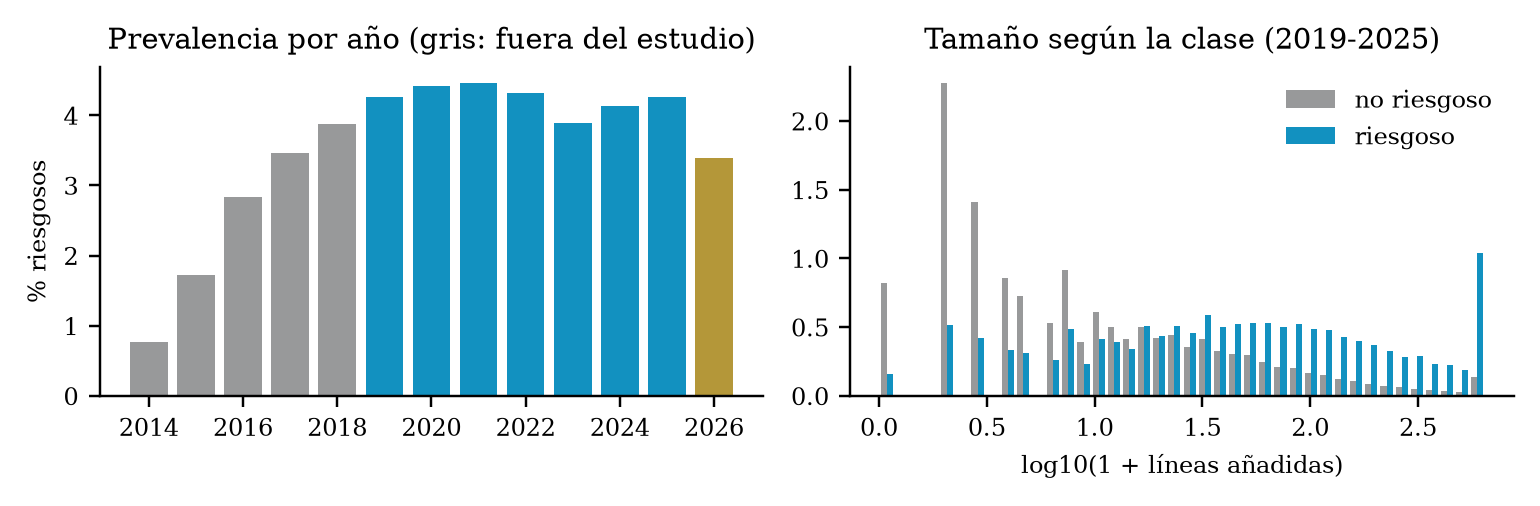
\includegraphics[width=\columnwidth]{../../resultados/e2/prevalencia_y_tamano.png}
\caption{Izquierda: prevalencia de commits riesgosos por año (en gris, los años fuera del estudio). Derecha: distribución del tamaño por clase en 2019--2025.}
\label{fig:eda}
\end{figure}

\subsection{Modelos y su papel}

La Tabla~\ref{tab:modelos} resume los modelos. Las dos referencias clásicas cubren dos extremos. La regresión logística es el estándar de JIT y es difícil de superar con partición temporal \cite{Kamei2013,Zeng2021}. El \emph{gradient boosting} \cite{Friedman2001} da la cota alta de una caja negra sobre las mismas variables.

\begin{table}[!t]
\caption{Modelos comparados}
\label{tab:modelos}
\centering\footnotesize
\begin{tabularx}{\columnwidth}{@{}l l Y@{}}
\toprule
\cabecera \textbf{Modelo} & \textbf{Papel} & \textbf{Justificación}\\
\midrule
Clase mayoritaria & Trivial & Su AUC-PR es la prevalencia: el piso\\
Reg.\ logística & Clásica & Estándar de JIT \cite{Kamei2013}; $\log(1+x)$ y estandarización\\
\emph{Gradient boosting} & Clásica fuerte & Cota alta sin restricción de interpretabilidad \cite{Friedman2001}\\
Difuso-evolutivo & Propuesto & $\le$15 reglas legibles; vértices y reglas ajustados con un AG\\
Difuso sin evolución & Variante de control & Mismas reglas iniciales, sin AG: mide el aporte de la evolución\\
\bottomrule
\end{tabularx}
\end{table}

\textbf{Qué propiedad de los datos aprovecha el modelo propuesto.} El riesgo crece por umbrales con el tamaño y la difusión, se modula con la revisión y la experiencia, y las variables tienen colas muy pesadas. Una partición difusa sobre la escala de cuantiles captura esos umbrales sin depender de la escala. Las reglas con pocos antecedentes capturan las interacciones que un mantenedor reconoce, por ejemplo ``si el cambio es grande y toca varios subsistemas''. El modelo usa 10 variables fijadas antes de ver resultados: líneas añadidas y borradas, archivos, subsistemas, \texttt{Reviewed-by}, \texttt{Signed-off-by}, si es corrección, si va a \emph{stable} y la experiencia del autor, en total y en el subsistema.

\subsection{Clasificador difuso-evolutivo}

Cada variable $x_j$ se lleva a $z_j\in[0,1]$ con su función de distribución empírica, estimada solo con el entrenamiento. Sobre $z_j$ se definen tres términos (bajo, medio, alto) que forman una partición de Ruspini \cite{Ruspini1969} con vértices $a_j<b_j<c_j$: bajo vale 1 hasta $a_j$ y cae a 0 en $b_j$; medio es el triángulo $(a_j,b_j,c_j)$; alto sube de 0 en $b_j$ a 1 en $c_j$. Una regla $r$ tiene hasta tres antecedentes y un peso $w_r\in[0,1]$:
\begin{equation}
\mu_r(\mathbf{x})=\prod_{(j,t)\in A_r}\mu_{jt}(z_j),\qquad
s(\mathbf{x})=1-\prod_{r}\bigl(1-w_r\,\mu_r(\mathbf{x})\bigr),
\end{equation}
es decir, t-norma producto y O probabilístico entre reglas. El puntaje $s$ ordena los commits por riesgo.

El ajuste sigue el enfoque Pittsburgh de los sistemas difusos genéticos \cite{Herrera2008,Ishibuchi2001}: cada individuo codifica todos los vértices y la base completa de reglas (activación, antecedentes, términos y pesos). La aptitud es el AUC-PR de entrenamiento, que es la métrica adecuada con clases desbalanceadas \cite{Saito2015}, menos una penalización por el número de antecedentes. Los operadores son:
\begin{itemize}
\item selección por torneo y elitismo;
\item cruce uniforme, que hereda cada regla completa;
\item mutación gaussiana de vértices y pesos, y mutación aleatoria de antecedentes y términos.
\end{itemize}

La variante sin evolución fija los vértices en los cuantiles $(0{,}2;\,0{,}5;\,0{,}8)$ y elige reglas de 1 o 2 antecedentes de forma voraz, por su confianza difusa, mientras mejore el AUC-PR. Esa misma solución siembra la población inicial del AG. Así, la diferencia entre ambas variantes aísla el aporte de la evolución.

\subsection{Pipeline sin fuga de información}

Todo lo que se aprende de los datos se ajusta solo con el entrenamiento de cada ventana y se aplica sin cambios a la validación o a la prueba:
\begin{itemize}
\item la transformación $\log(1+x)$ y la estandarización de la regresión logística, dentro de un \texttt{Pipeline};
\item la función de distribución empírica del modelo difuso;
\item el umbral de decisión.
\end{itemize}
No se balancean las clases: el AUC-PR se mide con la prevalencia real, y los conjuntos balanceados de forma artificial inflan el desempeño de manera engañosa \cite{Nguyen2025}. Las variables solo usan información anterior a la integración del commit. La experiencia del autor se cuenta con los commits previos en orden temporal.

\subsection{Partición temporal}

Nunca se mezclan commits al azar (Fig.~\ref{fig:particion}). Para cada año de validación $V\in\{2023,2024,2025\}$ se entrena con $[\text{2019-01-01},\ \text{inicio}(V)-90\text{ d})$ y se valida con el año $V$ completo. El hueco de 90 días replica lo que ocurre en la práctica: al entrenar, las etiquetas de los últimos 90 días todavía no existen. El modelo final se entrena con $[\text{2019-01-01},\ \text{2025-10-03})$ y se evalúa una sola vez con los \cifNPrueba{} commits de enero a julio de 2026 (prevalencia \cifPrevPrueba{}).

La partición de prueba quedó guardada con una huella SHA-256 de sus hashes y etiquetas. La evaluación final verifica de forma estricta que la huella no cambie. Se declara una salvedad: durante una fase preliminar de factibilidad, modelos simples se evaluaron una vez sobre 2026 para confirmar que había señal. Ninguna decisión posterior usó esas cifras.

\begin{figure}[!t]
\centering
% Partición temporal: ventana creciente con hueco de 90 días. Escala: 1 año = 0,85 cm desde 2019.
\begin{tikzpicture}[x=0.85cm,y=0.42cm,font=\scriptsize]
  \def\h{0.25}  % hueco de 90 días ~ 0,25 años
  \foreach \y/\lab/\ini in {3/V$_{2023}$/4, 2/V$_{2024}$/5, 1/V$_{2025}$/6}{
    \fill[udazul!70] (0,\y-0.32) rectangle (\ini-\h,\y+0.32);
    \fill[udplata!35] (\ini-\h,\y-0.32) rectangle (\ini,\y+0.32);
    \fill[uddorado!85] (\ini,\y-0.32) rectangle (\ini+1,\y+0.32);
    \node[left,udsable] at (0,\y) {\lab};
  }
  \fill[udazul!70] (0,-0.32) rectangle (7-\h,0.32);
  \fill[udplata!35] (7-\h,-0.32) rectangle (7,0.32);
  \fill[udrojo!80] (7,-0.32) rectangle (7+7/12,0.32);
  \node[left,udsable] at (0,0) {Prueba};
  \draw[udsable] (0,-0.75) -- (8,-0.75);
  \foreach \x/\t in {0/2019,1/2020,2/2021,3/2022,4/2023,5/2024,6/2025,7/2026}
    \draw[udsable] (\x,-0.75) -- ++(0,-0.12) node[below] {\t};
  \node[anchor=west,fill=udazul!70,minimum width=3mm,minimum height=2mm,inner sep=0] (a) at (0,4.2) {};
  \node[anchor=west] at (a.east) {entrenamiento};
  \node[anchor=west,fill=udplata!35,minimum width=3mm,minimum height=2mm,inner sep=0] (b) at (2.2,4.2) {};
  \node[anchor=west] at (b.east) {hueco 90 d};
  \node[anchor=west,fill=uddorado!85,minimum width=3mm,minimum height=2mm,inner sep=0] (c) at (4.1,4.2) {};
  \node[anchor=west] at (c.east) {validación};
  \node[anchor=west,fill=udrojo!80,minimum width=3mm,minimum height=2mm,inner sep=0] (d) at (5.9,4.2) {};
  \node[anchor=west] at (d.east) {prueba};
\end{tikzpicture}

\caption{Partición temporal con ventana creciente. Cada ventana de validación (2023, 2024 y 2025) se entrena con todo lo anterior menos un hueco de 90 días; la prueba (enero--julio de 2026) se evalúa una sola vez.}
\label{fig:particion}
\end{figure}

\subsection{Métricas y pruebas estadísticas}

\textbf{Métrica principal: AUC-PR} (precisión promedio de la clase riesgoso). Con una prevalencia cercana al 4\,\%, el AUC-ROC es engañosamente alto y el AUC-PR muestra la utilidad real de la lista de commits marcados \cite{Saito2015}. El AUC-PR de un clasificador sin información es igual a la prevalencia; por eso también se reporta el cociente AUC-PR/prevalencia.

\textbf{Métricas secundarias:} MCC, AUC-ROC, sensibilidad y especificidad. Las métricas que dependen de un umbral usan el que maximiza el MCC en la ventana de validación 2025, aplicado tal cual en la prueba.

\textbf{Costo:} tiempo de entrenamiento, tiempo de inferencia y número de parámetros.

\textbf{Incertidumbre.} Se reportan intervalos de confianza del 95\,\% por \emph{bootstrap} (1000 remuestreos de la prueba) y media $\pm$ desviación en 5 semillas (11, 23, 37, 41 y 53) para los modelos estocásticos.

\textbf{Pruebas.}
\begin{itemize}
\item McNemar con corrección de continuidad, entre el difuso-evolutivo y cada referencia, sobre las mismas predicciones de prueba \cite{Dietterich1998}.
\item Friedman con \emph{post hoc} de Nemenyi sobre los rangos de AUC-PR de los cinco modelos en las tres ventanas de validación más la prueba \cite{Demsar2006}.
\end{itemize}
En ambos casos $\alpha=0{,}05$. Con solo 5 semillas no se usa Wilcoxon. Una diferencia sin prueba se reporta como ``diferencia observada''.

\subsection{Resultados de validación de las referencias}

Las referencias se ajustaron con el mismo pipeline y la misma partición que el modelo propuesto. Se probó una pequeña rejilla (\cifNConfigsRef{} configuraciones) y se eligió la de mayor AUC-PR medio en las tres ventanas.

\textbf{Mejor referencia clásica:} el \emph{gradient boosting}, con AUC-PR medio de \cifValGB{} y alrededor de \cifParamGB{} parámetros (nodos de los árboles). Es la referencia $R$ del criterio de éxito.

\textbf{Regresión logística:} da \cifValLogistica{} con \cifParamLR{} parámetros, y la regularización no cambia nada porque hay cientos de miles de ejemplos.

\textbf{Clase mayoritaria:} queda en \cifValMayoritaria{}, la prevalencia. Ambas referencias clásicas la multiplican por cerca de cuatro.


\subsection{Espacio de hiperparámetros del modelo propuesto}

El espacio se declara antes de buscar (Tabla~\ref{tab:espacio}). La búsqueda es aleatoria, con 14 configuraciones de las 972 posibles. Cada configuración se evalúa en las tres ventanas con la semilla 11 y se elige por el AUC-PR medio. La sensibilidad se analiza sobre la rejilla de máximo de reglas $\times$ probabilidad de mutación, con el resto fijo en la mejor configuración. Después, la configuración elegida se entrena con las 5 semillas.

\begin{table}[!t]
\caption{Espacio de hiperparámetros del difuso-evolutivo}
\label{tab:espacio}
\centering\footnotesize
\begin{tabularx}{\columnwidth}{@{}l Y@{}}
\toprule
\cabecera \textbf{Hiperparámetro} & \textbf{Valores}\\
\midrule
\filas{../comun/tabla_espacio.tex}
\bottomrule
\end{tabularx}
\end{table}

%=====================================================================
\section{Experimentación}

Esta sección cubre el entrenamiento (fase F6). Todo se hizo sobre las ventanas de validación 2023--2025; la prueba de 2026 no interviene.

\subsection{Registro de experimentos}

El registro de experimentos guarda, de cada entrenamiento, la etapa, el modelo, la configuración, la semilla, la ventana, el tamaño de entrenamiento, el AUC-PR y el AUC-ROC de validación, el tiempo y el número de parámetros. Hay \cifRegReferencias{} corridas de las referencias y \cifRegPropuesto{} del modelo propuesto:
\begin{itemize}
\item \cifRegBusq{} de la búsqueda;
\item \cifRegSens{} de la sensibilidad;
\item 15 de las semillas;
\item 3 de la variante sin evolución.
\end{itemize}
Los entrenamientos corren en paralelo (6 procesos). Uno del difuso-evolutivo con la configuración final tarda unos \cifTiempoFE{} minutos con unos 450\,000 commits, porque la aptitud se evalúa sobre una muestra de 80\,000.

\subsection{Búsqueda aleatoria}

Se evaluaron \cifNBusqueda{} configuraciones del espacio de la Tabla~\ref{tab:espacio} en las tres ventanas. La mejor tiene la población y el número de generaciones más grandes del espacio y la mutación más baja, y alcanza un AUC-PR medio de \cifMejorBusqueda{}. Que gane el extremo del espacio sugiere que el AG aún tenía margen. No se amplió la búsqueda: se registra como limitación.


\subsection{Análisis de sensibilidad}

Con el resto fijo en la mejor configuración, se varió el máximo de reglas y la probabilidad de mutación (Fig.~\ref{fig:sensibilidad}).

\textbf{La mutación es lo que más pesa.} Con 0,05 el AUC-PR medio es \cifSensMutBaja{}; con 0,30 baja a \cifSensMutAlta{}. Una mutación alta destruye las reglas buenas antes de que se propaguen.

\textbf{El máximo de reglas casi no importa.} El mejor punto (\cifSensMaxR{} reglas, mutación \cifSensMaxPm{}) da \cifSensMax{}, prácticamente igual que con 5 o 15. El peor es \cifSensMinR{} reglas con mutación \cifSensMinPm{}, con \cifSensMin{}. Esto es coherente con lo que el AG hace en la práctica: aunque se le permitan 15 reglas, termina usando entre \cifReglasMin{} y \cifReglasMax{}.

La configuración congelada es la de la búsqueda (15 reglas como máximo). No se cambió a 10 después de ver la sensibilidad, porque la diferencia (0,001) está dentro de la variación entre semillas.

\begin{figure}[!t]
\centering
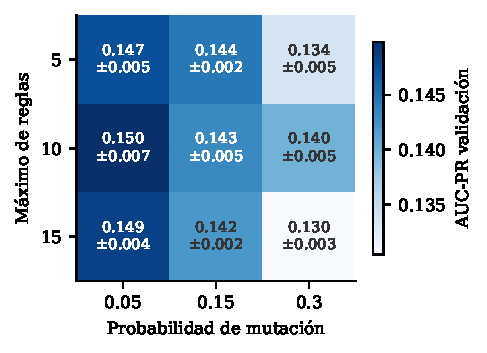
\includegraphics[width=0.82\columnwidth]{../../resultados/figuras/sensibilidad.pdf}
\caption{Sensibilidad: AUC-PR medio $\pm$ desviación en las tres ventanas, según el máximo de reglas y la probabilidad de mutación.}
\label{fig:sensibilidad}
\end{figure}

\subsection{Convergencia}

La Fig.~\ref{fig:convergencia} muestra la aptitud del mejor individuo y la mediana de la población, por generación, en la ventana 2025 para las 5 semillas. La mejora es rápida en las primeras 20 generaciones y se estabiliza entre la 60 y la 80. La distancia entre el mejor individuo y la mediana se mantiene, así que la población conserva diversidad hasta el final.

\begin{figure}[!t]
\centering
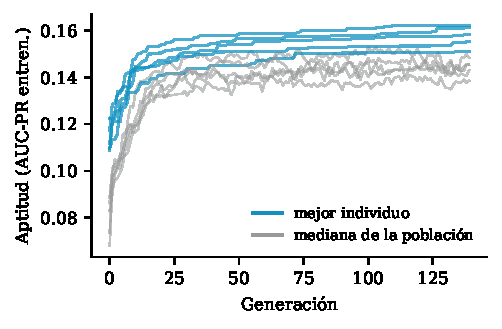
\includegraphics[width=0.92\columnwidth]{../../resultados/figuras/curva_aprendizaje.pdf}
\caption{Curva de aprendizaje del AG (ventana 2025, 5 semillas): aptitud del mejor individuo y mediana de la población.}
\label{fig:convergencia}
\end{figure}

\subsection{Semillas y aporte de la evolución}

La configuración elegida se entrenó con las 5 semillas (Tabla~\ref{tab:semillas}). El AUC-PR medio de validación es \cifValFE{} $\pm$ \cifValFEde{}. Es la diferencia observada respecto a las referencias, sin prueba de significancia todavía:
\begin{itemize}
\item prácticamente igual a la regresión logística (\cifValLogistica{});
\item el \cifRazonValFE{} del \emph{gradient boosting} (\cifValGB{});
\item muy por encima de la prevalencia.
\end{itemize}

La variante sin evolución arranca de la misma solución voraz y se queda en \cifValVariante{}. Usa \cifReglasVariante{} reglas con \cifAntVariante{} antecedentes. El AG no solo mejora el AUC-PR: también simplifica el modelo a entre \cifReglasMin{} y \cifReglasMax{} reglas, con \cifAntMin{} a \cifAntMax{} antecedentes en total.

\begin{table*}[!t]
\caption{Difuso-evolutivo con 5 semillas y variante sin evolución (validación)}
\label{tab:semillas}
\centering\footnotesize
\begin{tabular}{@{}l c c c c c c c@{}}
\toprule
\cabecera \textbf{Semilla} & \textbf{2023} & \textbf{2024} & \textbf{2025} & \textbf{Media} & \textbf{Reglas} & \textbf{Antec.} & \textbf{Tiempo (s)}\\
\midrule
\filas{../comun/tabla_semillas.tex}
\bottomrule
\end{tabular}
\end{table*}

\subsection{Configuración congelada}

Se congeló la configuración final antes de evaluar la prueba. Contiene:
\begin{itemize}
\item los hiperparámetros del difuso-evolutivo y las 5 semillas;
\item el umbral de MCC de cada semilla en la ventana 2025;
\item la semilla de referencia para McNemar (\cifSemillaRef{}, la de AUC-PR mediano);
\item la configuración y el umbral de cada referencia, con $R$ = \emph{gradient boosting};
\item la huella SHA-256 de la partición de prueba (\texttt{\cifHuella}\ldots).
\end{itemize}
El modelo final se entrena con todo 2019 hasta el 3 de octubre de 2025 y se evalúa una sola vez en 2026.

%=====================================================================
\section{Resultados en la prueba de 2026}

La configuración congelada se evaluó una sola vez sobre los \cifNPrueba{} commits de enero a julio de 2026 (prevalencia \cifPrevPrueba{}), tras verificar la huella de la partición. La Tabla~\ref{tab:prueba} reúne desempeño y costo.

\begin{table*}[!t]
\caption{Prueba de 2026: desempeño (media de las semillas; IC 95\,\% por \emph{bootstrap} de la semilla de referencia) y costo. Métricas con umbral: el que maximiza el MCC en 2025}
\label{tab:prueba}
\centering\footnotesize
\begin{tabular}{@{}l c c c c c c r r r@{}}
\toprule
\cabecera \textbf{Modelo} & \textbf{AUC-PR} & \textbf{IC 95\,\%} & \textbf{AUC-ROC} & \textbf{MCC} & \textbf{Sensib.} & \textbf{Especif.} & \textbf{Parám.} & \textbf{Entren.\ (s)} & \textbf{ms/1000}\\
\midrule
\filas{../comun/tabla_prueba.tex}
\bottomrule
\end{tabular}
\end{table*}

\subsection{Criterio de éxito}

El proyecto \textbf{no alcanza} el criterio fijado en la Entrega 1:
\begin{itemize}
\item \textbf{C1, desempeño: se cumple.} El difuso-evolutivo logra \cifTestFE{} $\pm$ \cifTestFEde{} de AUC-PR, el \cifCuno{} del \emph{gradient boosting} (\cifTestGB{}). La meta era 90\,\%.
\item \textbf{C2, robustez: no se cumple.} Pierde el \cifCaidaFE{} de su AUC-PR de validación; el \emph{gradient boosting} pierde el \cifCaidaGB{} y la regresión logística el \cifCaidaLR{}.
\item \textbf{C3, piso: se cumple solo en su primera parte.} El IC 95\,\% del AUC-PR, \cifTestFEic{}, excluye la prevalencia, y el modelo multiplica el AUC-PR del azar por cerca de 3,5. Las pruebas de McNemar son significativas ($p<10^{-6}$) contra todas las referencias, pero a favor de ellas, salvo contra la variante sin evolución:
  \begin{itemize}
  \item frente al \emph{gradient boosting}, el difuso acierta donde aquel falla en \cifMcAciertaGB{} commits y falla donde aquel acierta en \cifMcFallaGB{};
  \item frente a la variante sin evolución, las cifras se invierten: \cifMcAciertaVar{} frente a \cifMcFallaVar{}.
  \end{itemize}
\end{itemize}

\textbf{Friedman--Nemenyi.} La prueba de Friedman sobre los cuatro bloques (tres ventanas y la prueba) rechaza la igualdad de los cinco modelos ($p=\cifFriedmanP{}$). Los rangos medios son:
\begin{itemize}
\item \emph{gradient boosting}: \cifRangoGB{};
\item difuso-evolutivo y regresión logística: \cifRangoFE{};
\item variante sin evolución: \cifRangoVar{};
\item clase mayoritaria: \cifRangoMay{}.
\end{itemize}
Con la diferencia crítica de Nemenyi (\cifNemenyiCD{}), solo la distancia entre el \emph{gradient boosting} y la clase mayoritaria es significativa. Con cuatro bloques, la prueba tiene poca potencia.

\subsection{El umbral no se transfiere}

El AUC-PR del difuso-evolutivo es estable entre semillas (\cifFEApMin{}--\cifFEApMax{}). Sus métricas con umbral, en cambio, no lo son:
\begin{itemize}
\item el umbral fijado en 2025 marca entre el \cifFEMarcMin{} y el \cifFEMarcMax{} de los commits de 2026, según la semilla;
\item el MCC varía entre \cifFEMccMin{} y \cifFEMccMax{}.
\end{itemize}
La causa es estructural. Con 3 a 6 reglas, el puntaje toma pocos valores distintos, y un umbral elegido en una meseta de 2025 queda al borde de un escalón en 2026. Con la semilla de referencia marca el \cifFERefMarc{}, el doble que el \emph{gradient boosting}, y eso explica el McNemar desfavorable.

Las referencias, de puntaje continuo, conservan su tasa de marcado. Para ordenar commits por riesgo el modelo difuso sirve; para decidir con un corte fijo, su umbral debe recalibrarse con datos recientes.

\begin{figure}[!t]
\centering
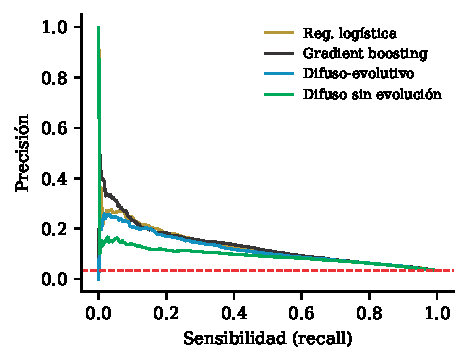
\includegraphics[width=0.9\columnwidth]{../../resultados/figuras/curvas_pr.pdf}
\caption{Curvas de precisión-sensibilidad en la prueba de 2026 (semilla de referencia). La línea roja es la prevalencia.}
\label{fig:pr}
\end{figure}

\subsection{Robustez y análisis de errores}

\textbf{Degradación dentro de 2026} (Fig.~\ref{fig:mes}). Todos los modelos se degradan a lo largo del año. El difuso-evolutivo baja de \cifMesIni{} en enero a \cifMesFin{} en julio, y el \emph{gradient boosting} de \cifMesGBIni{} a \cifMesGBFin{}. La deriva crece a medida que la prueba se aleja del entrenamiento.

\textbf{Subgrupo \texttt{Assisted-by}} (\cifAssistedN{} commits, prevalencia \cifAssistedPrev{}). Es descriptivo, porque la etiqueta es una cota inferior. Todos los modelos rinden peor que en el resto:
\begin{itemize}
\item difuso-evolutivo: \cifAssistedFE{} frente a \cifSinAssistedFE{};
\item \emph{gradient boosting}: \cifAssistedGB{} frente a \cifSinAssistedGB{};
\item regresión logística: \cifAssistedLR{} frente a \cifSinAssistedLR{}.
\end{itemize}
Las señales de tamaño y difusión que funcionan en general predicen menos en los commits declarados como asistidos.

\textbf{Errores por tipo de commit.} Los errores del difuso se concentran en dos grupos:
\begin{itemize}
\item \textbf{Commits pequeños.} En los tres quintiles inferiores de líneas añadidas la sensibilidad es 0: las reglas nunca los marcan. En el quintil superior (prevalencia \cifErrQcincoPrev{}) detecta el \cifErrQcincoSens{} de los riesgosos.
\item \textbf{Correcciones.} En los commits que traen su propio \texttt{Fixes:}, el AUC-PR es \cifErrFixAp{} frente a \cifErrNoFixAp{}, y la sensibilidad \cifErrFixSens{} frente a \cifErrNoFixSens{}. Una corrección que introduce otro error suele ser pequeña.
\end{itemize}

\begin{figure}[!t]
\centering
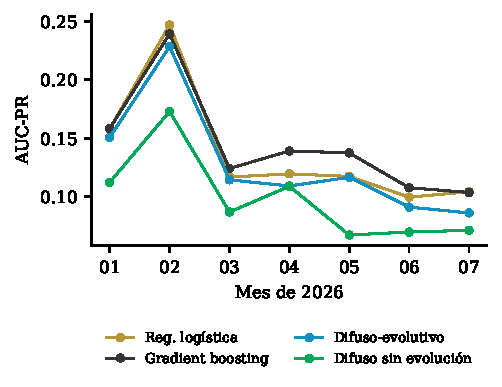
\includegraphics[width=0.95\columnwidth]{../../resultados/figuras/auc_pr_por_mes.pdf}
\caption{AUC-PR por mes de 2026 (semilla de referencia).}
\label{fig:mes}
\end{figure}

\subsection{Interpretabilidad: las reglas aprendidas}

El modelo de la semilla de referencia tiene \cifNReglasRef{} reglas (Tabla~\ref{tab:reglas}) y \cifParamFE{} parámetros en promedio entre semillas, frente a \cifParamGBprueba{} del \emph{gradient boosting}. Cada término se resume con su corte $\alpha=0{,}5$ en unidades originales.

Las reglas se leen solas:
\begin{itemize}
\item un cambio que agrega muchas líneas es sospechoso (R1), más aún si toca varios archivos (R2);
\item también lo es el que toca más de un subsistema (R4, R5);
\item con menos peso, el código nuevo puro: un solo subsistema y nada borrado (R3).
\end{itemize}
Coinciden con las familias de tamaño y difusión de la literatura JIT \cite{Kamei2013}. En esta semilla, la revisión (\texttt{Reviewed-by}) y la experiencia del autor no sobrevivieron a la evolución.

\begin{table}[!t]
\caption{Base de reglas del difuso-evolutivo (semilla de referencia). Entre paréntesis, el corte $\alpha=0{,}5$ de cada término}
\label{tab:reglas}
\centering\footnotesize
\begin{tabularx}{\columnwidth}{@{}c c Y@{}}
\toprule
\cabecera & \textbf{Peso} & \textbf{SI \ldots\ ENTONCES riesgoso}\\
\midrule
\filas{../comun/tabla_reglas.tex}
\bottomrule
\end{tabularx}
\end{table}

\textbf{Aporte de la evolución.} En la prueba, la evolución sube el AUC-PR un \cifAporteEvolPrueba{} frente a la variante sin evolución (\cifTestFE{} frente a \cifTestVar{}), y reduce el modelo de \cifReglasVariante{} reglas a 3--6.

%=====================================================================
\section{Iteración 2: vuelta al modelado}

CRISP-ML(Q) no es lineal: si la evaluación no alcanza el criterio, se vuelve a la preparación de datos o al modelado. Antes de correr nada se fijó un protocolo con el candidato, la regla de selección y la regla de adopción. El diagnóstico usa solo la validación y la exploración:
\begin{itemize}
\item la deriva de las covariables (más \texttt{Reviewed-by} y más correcciones con el tiempo) sugiere entrenar con una ventana deslizante de 3 años;
\item el difuso ve 10 de las 22 variables que usan las referencias, lo que sugiere un conjunto ampliado de 19.
\end{itemize}
El diseño es un factorial $2\times 2$ evaluado en validación. Cuando cambia la ventana, el \emph{gradient boosting} se reentrena con esa misma ventana.

Una regla de adopción evita usar la prueba otra vez sin necesidad: la iteración 2 solo se evaluaría en 2026 si su razón AUC-PR$_{FE}$/AUC-PR$_{GB}$ en validación superara la de la iteración 1 (\cifItDosUmbral{}).

\textbf{Resultado} (Fig.~\ref{fig:it2}): ningún candidato la supera.
\begin{itemize}
\item ventana creciente con 10 variables (la iteración 1): \cifItDosCreOriRazon{};
\item ventana deslizante con 10 variables: \cifItDosDesOriRazon{};
\item ventana creciente con 19 variables: \cifItDosCreAmpRazon{};
\item ventana deslizante con 19 variables: \cifItDosDesAmpRazon{}.
\end{itemize}
Más variables no ayudan: el AG sigue eligiendo 3 o 4 reglas de tamaño y difusión. Una ventana más corta tampoco cambia nada, y el \emph{gradient boosting} queda igual con ella.

La iteración 2 no se adoptó y la prueba no se volvió a usar. Las cifras de la Sección~V son las definitivas.

\begin{figure}[!t]
\centering
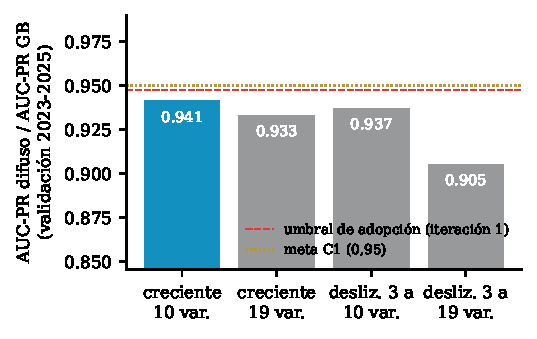
\includegraphics[width=0.88\columnwidth]{../../resultados/figuras/iteracion2_candidatos.pdf}
\caption{Iteración 2: razón de AUC-PR difuso/\emph{gradient boosting} en validación para los cuatro candidatos (semilla 11), frente al umbral de adopción.}
\label{fig:it2}
\end{figure}

%=====================================================================
\section{Discusión y limitaciones}

\textbf{El costo de la interpretabilidad es medible y moderado.} Con 3 a 6 reglas legibles y unos 27 parámetros, el modelo difuso conserva el \cifCuno{} del AUC-PR de un \emph{gradient boosting} con miles de nodos, y empata en rango medio con la regresión logística. La hipótesis de que la interpretabilidad intrínseca daría además robustez a la deriva no se sostiene: el difuso cae más que las referencias.

Una explicación consistente con los errores es que las reglas apuestan casi todo al tamaño y a la difusión. Cuando la deriva cambia la mezcla de commits (más correcciones pequeñas, más revisión), un modelo con pocas reglas no tiene con qué compensar.

\textbf{Amenazas a la validez.}
\begin{itemize}
\item \textbf{La prueba no estuvo intacta.} En la fase de factibilidad inicial se exploró 2026 con modelos simples. Ninguna decisión se basó en eso, pero la prueba no es virgen. La iteración 2 se decidió sin volver a evaluarla.
\item \textbf{La etiqueta.} \texttt{Fixes:} es fiable en torno al 81\,\% \cite{Lyu2024}. La censura de 90 días ignora los errores que se descubren más tarde \cite{Falessi2022}.
\item \textbf{El subgrupo \texttt{Assisted-by}} es una cota inferior: el 90\,\% de los commits asistidos no la declaraba \cite{KernelRemove}.
\item \textbf{Validez externa.} Se usó un solo proyecto.
\item \textbf{La búsqueda.} El mejor punto quedó en el extremo del espacio (población y generaciones máximas), así que podría haber margen.
\item \textbf{La iteración 2} comparó la semilla 11 contra un umbral calculado con 5 semillas. Aun con la semilla 11, ningún candidato superó a la iteración 1, así que la decisión no depende de esa asimetría.
\item \textbf{McNemar} compara aciertos con un umbral fijo y, con este desbalance, castiga a quien marca más. Por eso se complementa con el AUC-PR y sus intervalos.
\end{itemize}

%=====================================================================
\section{Conclusiones}

\begin{enumerate}
\item El clasificador difuso-evolutivo alcanzó la meta de desempeño de C1 al lograr en 2026 \cifTestFE{} de AUC-PR (\cifCuno{} del \emph{gradient boosting}, superando la meta del 90\,\%), aunque cayó \cifCaidaFE{} desde validación frente a \cifCaidaGB{} de la referencia.
\item Aun así, supera con amplio margen al azar (IC \cifTestFEic{} frente a una prevalencia de \cifPrevPrueba{}). Lo hace con \cifNReglasRef{} reglas que un mantenedor puede leer, frente a miles de parámetros.
\item La evolución es lo que hace útil al modelo: \cifAporteEvolPrueba{} más de AUC-PR que la variante sin evolución y, a la vez, de 15 a 3--6 reglas.
\item La debilidad práctica es el umbral. Con pocas reglas el puntaje es escalonado, y un corte fijado en 2025 no se transfiere a 2026. Recalibrarlo con datos recientes es el siguiente paso natural, junto con aptitudes que premien la estabilidad temporal.
\item Ninguno de los modelos predice bien los commits declarados como asistidos por IA (AUC-PR \cifAssistedFE{}--\cifAssistedLR{}), una pregunta abierta para cuando haya una etiqueta fiable.
\end{enumerate}


%=====================================================================
%=====================================================================
\section*{Declaración de uso de IA generativa}
{\footnotesize Usé Gemini para revisar y corregir errores y para redactar este informe a partir de los resultados del cuaderno y la recuperación de algunos papers para la evaluación del mismo.}


\section*{Anexo: reproducibilidad}
{\footnotesize Código, cuaderno ejecutado, registro de experimentos y configuración congelada se entregan con el artículo. Entorno: Python 3.13, pandas 3.1.1, scikit-learn 1.9.1, numpy 2.5.4, scipy 1.18.1. Semillas: 11, 23, 37, 41, 53 (modelos), 2026 (búsqueda), 1 y 2 (\emph{bootstrap}). El cuaderno de Colab parte de la tabla anonimizada, verifica la huella SHA-256 de la prueba (\texttt{\cifHuella}\ldots) y reproduce las cifras de la Tabla~\ref{tab:prueba}. \pendiente{Enlace público de la tabla de datos.}\par}

% Generado por revision/generar_e1.py final en orden de cita; no editar a mano.
\begin{thebibliography}{44}
\bibitem{Mockus2000} A. Mockus and D. M. Weiss, ``Predicting risk of software changes,'' Bell Labs Tech. J., vol. 5, no. 2, pp. 169--180, Apr.--Jun. 2000, doi: \mbox{10.1002/bltj.2229}.
\bibitem{Kamei2013} Y. Kamei, E. Shihab, B. Adams, A. E. Hassan, A. Mockus, A. Sinha, and N. Ubayashi, ``A large-scale empirical study of just-in-time quality assurance,'' IEEE Trans. Softw. Eng., vol. 39, no. 6, pp. 757--773, Jun. 2013, doi: \mbox{10.1109/TSE.2012.70}.
\bibitem{Sliwerski2005} J. Śliwerski, T. Zimmermann, and A. Zeller, ``When do changes induce fixes?'' in Proc. Int. Workshop Mining Softw. Repositories (MSR '05), St. Louis, MO, USA, 2005, pp. 1--5, doi: \mbox{10.1145/1083142.1083147}.
\bibitem{Lyu2024} Y. Lyu, H. J. Kang, R. Widyasari, J. Lawall, and D. Lo, ``Evaluating SZZ implementations: An empirical study on the Linux kernel,'' IEEE Trans. Softw. Eng., vol. 50, no. 9, pp. 2219--2239, Sep. 2024, doi: \mbox{10.1109/TSE.2024.3406718}.
\bibitem{KernelAdd} S. Levin, ``docs: add AI Coding Assistants documentation,'' Linux kernel, commit 78d979db6cef, Jan. 6, 2026. [Online]. Available: \url{https://github.com/torvalds/linux/commit/78d979db6cef}
\bibitem{KernelSimpl} C. Brauner, ``coding-assistants: simplify attribution,'' Linux kernel, commit 816d9992d9ed, Aug. 3, 2026. [Online]. Available: \url{https://github.com/torvalds/linux/commit/816d9992d9ed}
\bibitem{KernelRemove} S. Levin, ``docs: remove Assisted-by references,'' Linux kernel, commit 1e035297ffda, Oct. 14, 2026. [Online]. Available: \url{https://github.com/torvalds/linux/commit/1e035297ffda}
\bibitem{Studer2021} S. Studer, T. B. Bui, C. Drescher, A. Hanuschkin, L. Winkler, S. Peters, and K.-R. M\"uller, ``Towards CRISP-ML(Q): A machine learning process model with quality assurance methodology,'' Mach. Learn. Knowl. Extr., vol. 3, no. 2, pp. 392--413, 2021, doi: 10.3390/make3020020.
\bibitem{MaesBermejo2024} M. Maes Bermejo, J. M. González-Barahona, M. Gallego, and G. Robles, ``A dataset of Linux kernel commits'' (v3), Zenodo, 2024, doi: 10.5281/zenodo.10654193.
\bibitem{Page2021} M. J. Page \emph{et al.}, ``The PRISMA 2020 statement: An updated guideline for reporting systematic reviews,'' BMJ, vol. 372, Art. no. n71, 2021, doi: 10.1136/bmj.n71.
\bibitem{Zeng2021} Z. Zeng, Y. Zhang, H. Zhang, and L. Zhang, ``Deep just-in-time defect prediction: How far are we?'' in Proc. 30th ACM SIGSOFT Int. Symp. Softw. Testing Anal. (ISSTA), Virtual, Denmark, 2021, pp. 427--438, doi: \mbox{10.1145/3460319.3464819}.
\bibitem{Ni2022} C. Ni, W. Wang, K. Yang, X. Xia, K. Liu, and D. Lo, ``The best of both worlds: Integrating semantic features with expert features for defect prediction and localization,'' in Proc. 30th ACM Joint Eur. Softw. Eng. Conf. Symp. Found. Softw. Eng. (ESEC/FSE), Singapore, 2022, pp. 672--683, doi: \mbox{10.1145/3540250.3549165}.
\bibitem{Liu2026} Y. Liu, K. Jabre, R. Abreu, Z. J. Carmichael, V. Murali, A. Patel, J. Ge, W. Sun, C. Zhang, A. Mockus, D. Khavari, P. C. Rigby, and N. Nagappan, ``A preliminary study on explaining risk of code changes using LLM-based prediction models,'' in Proc. 3rd ACM Int. Conf. AI-Powered Softw. (AIware '26), Montreal, QC, Canada, 2026, pp. 259--267, doi: \mbox{10.1145/3805760.3814916}.
\bibitem{Jiarpakdee2021} J. Jiarpakdee, C. K. Tantithamthavorn, and J. Grundy, ``Practitioners' perceptions of the goals and visual explanations of defect prediction models,'' in Proc. IEEE/ACM 18th Int. Conf. Mining Softw. Repositories (MSR), 2021, pp. 432--443, doi: \mbox{10.1109/MSR52588.2021.00055}.
\bibitem{JITLine2021} C. Pornprasit and C. K. Tantithamthavorn, ``JITLine: A simpler, better, faster, finer-grained just-in-time defect prediction,'' in Proc. IEEE/ACM 18th Int. Conf. Mining Softw. Repositories (MSR), 2021, pp. 369--379, doi: \mbox{10.1109/MSR52588.2021.00049}.
\bibitem{PyExplainer2021} C. Pornprasit, C. Tantithamthavorn, J. Jiarpakdee, M. Fu, and P. Thongtanunam, ``PyExplainer: Explaining the predictions of just-in-time defect models,'' in Proc. 36th IEEE/ACM Int. Conf. Automated Softw. Eng. (ASE), 2021, pp. 407--418, doi: \mbox{10.1109/ASE51524.2021.9678763}.
\bibitem{Sahar2024} H. Sahar, A. A. Bangash, A. Hindle, and D. Barbosa, ``IRJIT: A simple, online, information retrieval approach for just-in-time software defect prediction,'' Empir. Softw. Eng., vol. 29, no. 5, Art. no. 131, 2024, doi: \mbox{10.1007/s10664-024-10514-z}.
\bibitem{Yu2024FoX} J. Yu, M. Fu, A. Ignatiev, C. Tantithamthavorn, and P. Stuckey, ``A formal explainer for just-in-time defect predictions,'' ACM Trans. Softw. Eng. Methodol., vol. 33, no. 7, pp. 1--31, Sep. 2024, doi: \mbox{10.1145/3664809}.
\bibitem{Chen2018MULTI} X. Chen, Y. Zhao, Q. Wang, and Z. Yuan, ``MULTI: Multi-objective effort-aware just-in-time software defect prediction,'' Inf. Softw. Technol., vol. 93, pp. 1--13, Jan. 2018, doi: \mbox{10.1016/j.infsof.2017.08.004}.
\bibitem{Kang2021} J. Kang, S. Kwon, D. Ryu, and J. Baik, ``HASPO: Harmony search-based parameter optimization for just-in-time software defect prediction in maritime software,'' Appl. Sci., vol. 11, no. 5, Art. no. 2002, 2021, doi: \mbox{10.3390/app11052002}.
\bibitem{Mostafa2025} S. Mostafa, S. T. Cynthia, B. Roy, and D. Mondal, ``Feature transformation for improved software bug detection and commit classification,'' J. Syst. Softw., vol. 219, Art. no. 112205, Jan. 2025, doi: \mbox{10.1016/j.jss.2024.112205}.
\bibitem{Chen2025} F. Chen, Y. Ke, X. Liu, and Q. Wei, ``Multi-project just-in-time software defect prediction based on multi-task learning for mobile applications,'' in Proc. IEEE Conf. Softw. Testing, Verification Validation (ICST), 2025, pp. 127--137, doi: \mbox{10.1109/ICST62969.2025.10989004}.
\bibitem{Aftab2023} S. Aftab, S. Abbas, T. M. Ghazal, M. Ahmad, H. A. Hamadi, C. Y. Yeun, and M. A. Khan, ``A cloud-based software defect prediction system using data and decision-level machine learning fusion,'' Mathematics, vol. 11, no. 3, Art. no. 632, 2023, doi: \mbox{10.3390/math11030632}.
\bibitem{Dey2025} R. Dey, J. Piri, B. Acharya, P. P. Das, V. C. Gerogiannis, and A. Kanavos, ``A hybrid evolutionary fuzzy ensemble approach for accurate software defect prediction,'' Mathematics, vol. 13, no. 7, Art. no. 1140, 2025, doi: \mbox{10.3390/math13071140}.
\bibitem{McIntosh2018} S. McIntosh and Y. Kamei, ``Are fix-inducing changes a moving target? A longitudinal case study of just-in-time defect prediction,'' IEEE Trans. Softw. Eng., vol. 44, no. 5, pp. 412--428, May 2018, doi: \mbox{10.1109/TSE.2017.2693980}.
\bibitem{Shehab2023} M. A. Shehab, A. Hamou-Lhadj, and V. S. P. Gunda, ``JITBoost: Boosting just-in-time defect prediction using Boolean combination of classifiers,'' in Proc. IEEE 23rd Int. Conf. Softw. Qual., Rel. Secur. (QRS), 2023, pp. 95--104, doi: \mbox{10.1109/QRS60937.2023.00019}.
\bibitem{Chitsazian2026} Z. Chitsazian, S. Sedighian Kashi, and A. Nikanjam, ``Detecting concept drift in just-in-time software defect prediction using model interpretation,'' Int. J. Syst. Assur. Eng. Manag., vol. 17, no. 9, pp. 2701--2722, 2026, doi: \mbox{10.1007/s13198-025-03122-7}.
\bibitem{Patel2024} H. J. Patel, B. Adams, and A. E. Hassan, ``Post deployment recycling of machine learning models,'' Empir. Softw. Eng., vol. 29, no. 4, Art. no. 100, 2024, doi: \mbox{10.1007/s10664-024-10492-2}.
\bibitem{Olewicki2024} D. Olewicki, S. Habchi, M. Nayrolles, M. Faramarzi, S. Chandar, and B. Adams, ``On the costs and benefits of adopting lifelong learning for software analytics -- Empirical study on brown build and risk prediction,'' in Proc. 46th Int. Conf. Softw. Eng.: Softw. Eng. Pract. (ICSE-SEIP), Lisbon, Portugal, 2024, pp. 275--286, doi: \mbox{10.1145/3639477.3639717}.
\bibitem{Tian2026} D. Tian, L. Song, and X. Su, ``Just-in-time quality assurance with assistance of automated defect prediction and code testing,'' ACM Trans. Softw. Eng. Methodol., vol. 35, no. 9, pp. 1--46, 2026, doi: \mbox{10.1145/3779653}.
\bibitem{Cabral2019} G. G. Cabral, L. L. Minku, E. Shihab, and S. Mujahid, ``Class imbalance evolution and verification latency in just-in-time software defect prediction,'' in Proc. IEEE/ACM 41st Int. Conf. Softw. Eng. (ICSE), Montreal, QC, Canada, 2019, pp. 666--676, doi: \mbox{10.1109/ICSE.2019.00076}.
\bibitem{Song2023} L. Song and L. L. Minku, ``A procedure to continuously evaluate predictive performance of just-in-time software defect prediction models during software development,'' IEEE Trans. Softw. Eng., vol. 49, no. 2, pp. 646--666, Feb. 2023, doi: \mbox{10.1109/TSE.2022.3158831}.
\bibitem{Nguyen2025} D. Nguyen, T. Le-Cong, T. H. M. Le, M. A. Babar, and Q.-T. Huynh, ``Toward realistic evaluations of just-in-time vulnerability prediction,'' in Proc. IEEE Int. Conf. Softw. Maint. Evol. (ICSME), Auckland, New Zealand, 2025, pp. 1--10, doi: \mbox{10.1109/ICSME64153.2025.00023}.
\bibitem{Mazloomzadeh2026} I. Mazloomzadeh, M. M. Morovati, and F. Khomh, ``How do AI coding agents contribute to software development? An empirical study of agentic pull requests,'' arXiv:2607.21832, Jul. 2026, doi: \mbox{10.48550/arXiv.2607.21832}.
\bibitem{Herbold2022} S. Herbold, A. Trautsch, F. Trautsch, and B. Ledel, ``Problems with SZZ and features: An empirical study of the state of practice of defect prediction data collection,'' Empir. Softw. Eng., vol. 27, no. 2, Art. no. 42, 2022, doi: \mbox{10.1007/s10664-021-10092-4}.
\bibitem{Veras2025} R. C. Veras, G. G. Cabral, and A. L. I. de Oliveira, ``Semantic SZZ: Mitigating the impact of misclassified corrective changes in just-in-time software defect prediction,'' in Proc. IEEE Int. Conf. Syst., Man, Cybern. (SMC), 2025, pp. 769--774, doi: \mbox{10.1109/SMC58881.2025.11342537}.
\bibitem{Falessi2022} D. Falessi, A. Ahluwalia, and M. Di Penta, ``The impact of dormant defects on defect prediction: A study of 19 Apache projects,'' ACM Trans. Softw. Eng. Methodol., vol. 31, no. 1, pp. 1--26, Jan. 2022, doi: \mbox{10.1145/3467895}.
\bibitem{Friedman2001} J. H. Friedman, ``Greedy function approximation: A gradient boosting machine,'' Ann. Statist., vol. 29, no. 5, pp. 1189--1232, Oct. 2001, doi: \mbox{10.1214/aos/1013203451}.
\bibitem{Ruspini1969} E. H. Ruspini, ``A new approach to clustering,'' Inf. Control, vol. 15, no. 1, pp. 22--32, Jul. 1969, doi: \mbox{10.1016/S0019-9958(69)90591-9}.
\bibitem{Herrera2008} F. Herrera, ``Genetic fuzzy systems: taxonomy, current research trends and prospects,'' Evol. Intell., vol. 1, no. 1, pp. 27--46, Mar. 2008, doi: \mbox{10.1007/s12065-007-0001-5}.
\bibitem{Ishibuchi2001} H. Ishibuchi, T. Nakashima, and T. Murata, ``Three-objective genetics-based machine learning for linguistic rule extraction,'' Inf. Sci., vol. 136, no. 1--4, pp. 109--133, Aug. 2001, doi: \mbox{10.1016/S0020-0255(01)00144-X}.
\bibitem{Saito2015} T. Saito and M. Rehmsmeier, ``The precision-recall plot is more informative than the ROC plot when evaluating binary classifiers on imbalanced datasets,'' PLOS ONE, vol. 10, no. 3, Art. no. e0118432, Mar. 2015, doi: \mbox{10.1371/journal.pone.0118432}.
\bibitem{Dietterich1998} T. G. Dietterich, ``Approximate statistical tests for comparing supervised classification learning algorithms,'' Neural Comput., vol. 10, no. 7, pp. 1895--1923, Oct. 1998, doi: \mbox{10.1162/089976698300017197}.
\bibitem{Demsar2006} J. Demšar, ``Statistical comparisons of classifiers over multiple data sets,'' J. Mach. Learn. Res., vol. 7, pp. 1--30, 2006. [Online]. Available: \url{https://jmlr.org/papers/v7/demsar06a.html}
\end{thebibliography}


\end{document}
